\documentclass[11pt,]{article}
\usepackage{lmodern}
\usepackage{amssymb,amsmath}
\usepackage{ifxetex,ifluatex}
\usepackage{fixltx2e} % provides \textsubscript
\ifnum 0\ifxetex 1\fi\ifluatex 1\fi=0 % if pdftex
  \usepackage[T1]{fontenc}
  \usepackage[utf8]{inputenc}
\else % if luatex or xelatex
  \ifxetex
    \usepackage{mathspec}
  \else
    \usepackage{fontspec}
  \fi
  \defaultfontfeatures{Ligatures=TeX,Scale=MatchLowercase}
\fi
% use upquote if available, for straight quotes in verbatim environments
\IfFileExists{upquote.sty}{\usepackage{upquote}}{}
% use microtype if available
\IfFileExists{microtype.sty}{%
\usepackage{microtype}
\UseMicrotypeSet[protrusion]{basicmath} % disable protrusion for tt fonts
}{}
\usepackage[margin=3cm]{geometry}
\usepackage{hyperref}
\hypersetup{unicode=true,
            pdftitle={An introduction to R for ecological modeling (lab 1)},
            pdfauthor={Stephen Ellner, modified by Ben Bolker. Adapted to R Markdown by Alejandro Morales},
            pdfborder={0 0 0},
            breaklinks=true}
\urlstyle{same}  % don't use monospace font for urls
\usepackage{color}
\usepackage{fancyvrb}
\newcommand{\VerbBar}{|}
\newcommand{\VERB}{\Verb[commandchars=\\\{\}]}
\DefineVerbatimEnvironment{Highlighting}{Verbatim}{commandchars=\\\{\}}
% Add ',fontsize=\small' for more characters per line
\usepackage{framed}
\definecolor{shadecolor}{RGB}{248,248,248}
\newenvironment{Shaded}{\begin{snugshade}}{\end{snugshade}}
\newcommand{\KeywordTok}[1]{\textcolor[rgb]{0.13,0.29,0.53}{\textbf{#1}}}
\newcommand{\DataTypeTok}[1]{\textcolor[rgb]{0.13,0.29,0.53}{#1}}
\newcommand{\DecValTok}[1]{\textcolor[rgb]{0.00,0.00,0.81}{#1}}
\newcommand{\BaseNTok}[1]{\textcolor[rgb]{0.00,0.00,0.81}{#1}}
\newcommand{\FloatTok}[1]{\textcolor[rgb]{0.00,0.00,0.81}{#1}}
\newcommand{\ConstantTok}[1]{\textcolor[rgb]{0.00,0.00,0.00}{#1}}
\newcommand{\CharTok}[1]{\textcolor[rgb]{0.31,0.60,0.02}{#1}}
\newcommand{\SpecialCharTok}[1]{\textcolor[rgb]{0.00,0.00,0.00}{#1}}
\newcommand{\StringTok}[1]{\textcolor[rgb]{0.31,0.60,0.02}{#1}}
\newcommand{\VerbatimStringTok}[1]{\textcolor[rgb]{0.31,0.60,0.02}{#1}}
\newcommand{\SpecialStringTok}[1]{\textcolor[rgb]{0.31,0.60,0.02}{#1}}
\newcommand{\ImportTok}[1]{#1}
\newcommand{\CommentTok}[1]{\textcolor[rgb]{0.56,0.35,0.01}{\textit{#1}}}
\newcommand{\DocumentationTok}[1]{\textcolor[rgb]{0.56,0.35,0.01}{\textbf{\textit{#1}}}}
\newcommand{\AnnotationTok}[1]{\textcolor[rgb]{0.56,0.35,0.01}{\textbf{\textit{#1}}}}
\newcommand{\CommentVarTok}[1]{\textcolor[rgb]{0.56,0.35,0.01}{\textbf{\textit{#1}}}}
\newcommand{\OtherTok}[1]{\textcolor[rgb]{0.56,0.35,0.01}{#1}}
\newcommand{\FunctionTok}[1]{\textcolor[rgb]{0.00,0.00,0.00}{#1}}
\newcommand{\VariableTok}[1]{\textcolor[rgb]{0.00,0.00,0.00}{#1}}
\newcommand{\ControlFlowTok}[1]{\textcolor[rgb]{0.13,0.29,0.53}{\textbf{#1}}}
\newcommand{\OperatorTok}[1]{\textcolor[rgb]{0.81,0.36,0.00}{\textbf{#1}}}
\newcommand{\BuiltInTok}[1]{#1}
\newcommand{\ExtensionTok}[1]{#1}
\newcommand{\PreprocessorTok}[1]{\textcolor[rgb]{0.56,0.35,0.01}{\textit{#1}}}
\newcommand{\AttributeTok}[1]{\textcolor[rgb]{0.77,0.63,0.00}{#1}}
\newcommand{\RegionMarkerTok}[1]{#1}
\newcommand{\InformationTok}[1]{\textcolor[rgb]{0.56,0.35,0.01}{\textbf{\textit{#1}}}}
\newcommand{\WarningTok}[1]{\textcolor[rgb]{0.56,0.35,0.01}{\textbf{\textit{#1}}}}
\newcommand{\AlertTok}[1]{\textcolor[rgb]{0.94,0.16,0.16}{#1}}
\newcommand{\ErrorTok}[1]{\textcolor[rgb]{0.64,0.00,0.00}{\textbf{#1}}}
\newcommand{\NormalTok}[1]{#1}
\usepackage{graphicx,grffile}
\makeatletter
\def\maxwidth{\ifdim\Gin@nat@width>\linewidth\linewidth\else\Gin@nat@width\fi}
\def\maxheight{\ifdim\Gin@nat@height>\textheight\textheight\else\Gin@nat@height\fi}
\makeatother
% Scale images if necessary, so that they will not overflow the page
% margins by default, and it is still possible to overwrite the defaults
% using explicit options in \includegraphics[width, height, ...]{}
\setkeys{Gin}{width=\maxwidth,height=\maxheight,keepaspectratio}
\IfFileExists{parskip.sty}{%
\usepackage{parskip}
}{% else
\setlength{\parindent}{0pt}
\setlength{\parskip}{6pt plus 2pt minus 1pt}
}
\setlength{\emergencystretch}{3em}  % prevent overfull lines
\providecommand{\tightlist}{%
  \setlength{\itemsep}{0pt}\setlength{\parskip}{0pt}}
\setcounter{secnumdepth}{5}
% Redefines (sub)paragraphs to behave more like sections
\ifx\paragraph\undefined\else
\let\oldparagraph\paragraph
\renewcommand{\paragraph}[1]{\oldparagraph{#1}\mbox{}}
\fi
\ifx\subparagraph\undefined\else
\let\oldsubparagraph\subparagraph
\renewcommand{\subparagraph}[1]{\oldsubparagraph{#1}\mbox{}}
\fi

%%% Use protect on footnotes to avoid problems with footnotes in titles
\let\rmarkdownfootnote\footnote%
\def\footnote{\protect\rmarkdownfootnote}

%%% Change title format to be more compact
\usepackage{titling}

% Create subtitle command for use in maketitle
\newcommand{\subtitle}[1]{
  \posttitle{
    \begin{center}\large#1\end{center}
    }
}

\setlength{\droptitle}{-2em}

  \title{An introduction to \texttt{R} for ecological modeling (lab 1)}
    \pretitle{\vspace{\droptitle}\centering\huge}
  \posttitle{\par}
    \author{Stephen Ellner, modified by Ben Bolker. Adapted to R Markdown by
Alejandro Morales}
    \preauthor{\centering\large\emph}
  \postauthor{\par}
      \predate{\centering\large\emph}
  \postdate{\par}
    \date{October 8, 2018}

\usepackage{booktabs}
\usepackage{longtable}
\usepackage{array}
\usepackage{multirow}
\usepackage[table]{xcolor}
\usepackage{wrapfig}
\usepackage{float}
\usepackage{colortbl}
\usepackage{pdflscape}
\usepackage{tabu}
\usepackage{threeparttable}
\usepackage{threeparttablex}
\usepackage[normalem]{ulem}
\usepackage{makecell}

\begin{document}
\maketitle

\section{How to use this document}\label{how-to-use-this-document}

\begin{itemize}
\item
  These notes contain many sample calculations. It is important to do
  these yourself---\textbf{type them in at your keyboard and see what
  happens on your screen}---to get the feel of working in R.
\item
  \textbf{Exercises} in the middle of a section should be done
  immediately when you get to them, and make sure you have them right
  before moving on. Some more challenging exercises (indicated by
  asterisks) appear at the end of some sections. These can be left until
  later, and may be assigned as homework.
\end{itemize}

These notes are based in part on course materials by former TAs Colleen
Webb, Jonathan Rowell and Daniel Fink at Cornell, Professors Lou Gross
(University of Tennessee) and Paul Fackler (NC State University), and on
the book \emph{Getting Started with Matlab} by Rudra Pratap (Oxford
University Press). They also draw on the documentation supplied with R.
They parallel, but go into more depth than, the chapter supplement for
the book \emph{Ecological Models and Data in R}.

You can find many other similar introductions scattered around the web,
or in the ``contributed documentation'' section on the R web site
(\url{http://cran.r-project.org/other-docs.html}). This particular
version is limited (it has similar coverage to Sections 1 and 2 of the
\emph{Introduction to R} that comes with R) and targets biologists who
are neither programmers nor statisticians.

\section{What is R?}\label{what-is-r}

R is an object-oriented scripting language that combines

\begin{itemize}
\item
  a programming language called Slang, developed by John Chambers at
  Bell Labs, that can be used for numerical simulation of deterministic
  and stochastic dynamic models
\item
  an extensive set of functions for classical and modern statistical
  data analysis and modeling
\item
  graphics functions for visualizing data and model output
\item
  a user interface with a few basic menus and extensive help facilities
\end{itemize}

R is an open source project, available for free download via the Web.
Originally a research project in statistical computing (Ihaka and
Gentleman, 1996, it is now managed by a development team that includes a
number of well-regarded statisticians, and is widely used by statistical
researchers (and a growing number of theoretical ecologists and
ecological modelers) as a platform for making new methods available to
users. The commercial implementation of Slang (called S-PLUS) offers an
Office-style ``point and click''" interface that R lacks. For our
purposes, however, the advantage of this front-end is outweighed by the
fact that R is built on a faster and much less memory-hungry
implementation of Slang and is easier to interface with other languages
(and is free!). A standard installation of R also includes extensive
documentation, including an introductory manual (\(\approx 100\) pages)
and a comprehensive reference manual (over 1000 pages). (There is a
graphical front-end for parts of R, called ``R commander'' (Rcmdr for
short), available at the R site, but we will not be using it in this
class.)

\subsection{Installing R on your computer:
basics}\label{installing-r-on-your-computer-basics}

If R is already installed on your computer, you can skip this section.

The main source for R is the CRAN home page
\texttt{http://cran.r-project.org}. You can get the source code, but
most users will prefer a precompiled version. To get one of these from
CRAN:

\begin{itemize}
\item
  go to \texttt{http://cran.r-project.org/mirrors.html} and find a
  mirror site that is geographically somewhat near you.
\item
  Find the appropriate page for your operating system --- when you get
  to the download section, go to \texttt{base} rather than
  \texttt{contrib}. Download the binary file (e.g.
  \texttt{base/R-x.y.z-win32.exe} for Windows, \texttt{R-x.y.z.dmg} for
  MacOS, where \texttt{x.y.z} is the version number). The binary files
  are large (30--60 megabytes) --- you will need to find a fast internet
  connection.
\item
  Read and follow the instructions (which are pretty much ``click on the
  icon'').
\end{itemize}

R should work well on any reasonably modern computer. Version 2.5.1
requires MacOS X 10.4.4 (or higher) or Windows 95 (or higher), or just
about any version of Linux; it can also be compiled on other versions of
Unix. Windows XP or higher is recommended. R moves quickly: if possible,
you should make sure you have upgraded to the most recent version
available, or at least that your version isn't more than about a year
old.

The standard distributions of R include several \emph{packages},
user-contributed suites of add-on functions (unfortunately, the command
to load a package into R is \texttt{library}!). These Notes use some
packages that are not part of the standard distribution. In general, you
can install additional packages from within R using the
\texttt{Packages} menu, or the \texttt{install.packages} command. (See
below.)

For Windows or MacOS, install R by launching the downloaded file and
following the on-screen instructions. At the end you'll have an R icon
on your desktop that you can use to launch the program. Installing
versions for Linux or Unix is slightly more complicated, which will not
bother the corresponding users. For doing anything more than very simple
examples, we recommend the Tinn-R
(\texttt{http://www.sci-views.org/Tinn-R}) or Notepad++
(\texttt{notepad-plus.sourceforge.net/}) editors as better Windows
interfaces than the built-in console: in particular, these editors have
\emph{syntax highlighting}, which colors R commands and allows you to
identify missing parentheses, quotation marks, etc..

Windows: If you are using R on a machine where you have sufficient
permissions, you may want to edit some of your graphical user interface
(GUI) options.

\begin{itemize}
\item
  To allow command and graphics windows to move independently on the
  desktop (SDI, single-document interface, rather than MDI,
  multiple-document interface): go to \texttt{File/Edit/Preferences} and
  click the radio button to set \texttt{SDI} instead of \texttt{MDI}.
  This edits the \texttt{Rconsole} file. R~will ask you where to save
  it; click through to \texttt{My\ Computer/Program\ Files/R/R-x.y.z/},
  where \texttt{x.y.z} stands for the version of R. You will then need
  to restart R.
\item
  To select the most powerful version of the help system, go to the same
  directory (\texttt{My\ Computer/Program\ Files/R/R-x.y.z/}) and use
  Notepad to edit the \texttt{Rprofile} file to un-comment
  \texttt{options(chmhelp=TRUE)} by removing the \# at the start of the
  line.
\end{itemize}

\subsection{Starting R}\label{starting-r}

Windows: Just click on the icon on your desktop, or in the
\texttt{Start} menu (if you allowed the Setup program to make either or
both of these). If you lose these shortcuts for some reason, you can
search for the executable file \texttt{Rgui.exe} on your hard drive,
which will probably be somewhere like
\texttt{Program\ Files\textbackslash{}R\textbackslash{}R-x.y.z\textbackslash{}bin\textbackslash{}Rgui.exe}.
If you are using \texttt{Tinn-R}, first start \texttt{Tinn-R}, then go
to \ldots{}

\subsection{Stopping R}\label{stopping-r}

You can stop R from the \texttt{File} menu (Windows), or you can stop it
by typing \texttt{q()} at the command prompt (if you type \texttt{q} by
itself, you will get some confusing output which is actually R trying to
tell you the definition of the \texttt{q} function; more on this later).

When you quit, R will ask you if you want to save the workspace (that
is, all of the variables you have defined in this session); for now (and
in general), say ``no'' in order to avoid clutter.

Should an R command seem to be stuck or take longer than you're willing
to wait, click on the stop sign on the menu bar or hit the
\texttt{Escape} key (in Unix, type Control-C).

\section{Interactive calculations}\label{interactive-calculations}

Windows: When you start R it opens the \textbf{console} window. The
console has a few basic menus at the top; check them out on your own.
The console is also where you enter commands for R to execute
\emph{interactively}, meaning that the command is executed and the
result is displayed as soon as you hit the \texttt{Enter} key. For
example, at the command prompt \texttt{\textgreater{}}, type in
\texttt{2+2} and hit \texttt{Enter}; you will see

\begin{Shaded}
\begin{Highlighting}[]
\DecValTok{2}\OperatorTok{+}\DecValTok{2} 
\end{Highlighting}
\end{Shaded}

\begin{verbatim}
## [1] 4
\end{verbatim}

To do anything complicated, you have to store the results from
calculations by \emph{assigning} them to variables, using \texttt{=} or
\texttt{\textless{}-}. For example:

\begin{Shaded}
\begin{Highlighting}[]
\NormalTok{a=}\DecValTok{2}\OperatorTok{+}\DecValTok{2}
\end{Highlighting}
\end{Shaded}

R automatically creates the variable \texttt{a} and stores the result
(4) in it, but it doesn't print anything. This may seem strange, but
you'll often be creating and manipulating huge sets of data that would
fill many screens, so the default is to skip printing the results. To
ask R to print the value, just type the variable name by itself at the
command prompt:

\begin{Shaded}
\begin{Highlighting}[]
\NormalTok{a}
\end{Highlighting}
\end{Shaded}

\begin{verbatim}
## [1] 4
\end{verbatim}

(the \texttt{{[}1{]}} at the beginning of the line is just R printing an
index of element numbers; if you print a result that displays on
multiple lines, R will put an index at the beginning of each line.
\texttt{print(a)} also works to print the value of a variable.) By
default, a variable created this way is a \emph{vector}, and it is
\emph{numeric} because we gave R a number rather than some other type of
data (e.g.~a character string like \texttt{"pxqr"}). In this case
\texttt{a} is a numeric vector of length 1, which acts just like a
number.

You could also type \texttt{a=2+2;\ a}, using a semicolon to put two or
more commands on a single line. Conversely, you can break lines
\emph{anywhere that R can tell you haven't finished your command} and R
will give you a ``continuation'' prompt (\texttt{+}) to let you know
that it doesn't think you're finished yet: try typing

\begin{Shaded}
\begin{Highlighting}[]
\NormalTok{a=}\DecValTok{3}\OperatorTok{*}\NormalTok{(}\DecValTok{4}\OperatorTok{+}\StringTok{ }\NormalTok{[Enter]}
\DecValTok{5}\NormalTok{)}
\end{Highlighting}
\end{Shaded}

to see what happens (you will sometimes see the continuation prompt when
you don't expect it, e.g.~if you forget to close parentheses). If you
get stuck continuing a command you don't want---e.g.~you opened the
wrong parentheses---just hit the \texttt{Escape} key or the stop icon in
the menu bar to get out.

Variable names in R must begin with a letter, followed by letters or
numbers. You can break up long names with a period, as in
\texttt{very.long.variable.number.3}, or an underscore (\texttt{\_}),
but you can't use blank spaces in variable names (or at least it's not
worth the trouble). Variable names in R are case sensitive, so
\texttt{Abc} and \texttt{abc} are different variables. Make variable
names long enough to remember, short enough to type.\texttt{N.per.ha} or
\texttt{pop.density} are better than \texttt{x} and \texttt{y} (too
short) or \texttt{available.nitrogen.per.hectare} (too long). Avoid
\texttt{c}, \texttt{l}, \texttt{q}, \texttt{t}, \texttt{C}, \texttt{D},
\texttt{F}, \texttt{I}, and \texttt{T}, which are either built-in R
functions or hard to tell apart.

R does calculations with variables as if they were numbers. It uses
\texttt{+}, \texttt{-}, \texttt{*}, \texttt{/}, and \texttt{\^{}} for
addition, subtraction, multiplication, division and exponentiation,
respectively. For example:

\begin{Shaded}
\begin{Highlighting}[]
\NormalTok{x=}\DecValTok{5}
\NormalTok{y=}\DecValTok{2}
\NormalTok{z1=x}\OperatorTok{*}\NormalTok{y ## no output}
\NormalTok{z2=x}\OperatorTok{/}\NormalTok{y ## no output}
\NormalTok{z3=x}\OperatorTok{^}\NormalTok{y ## no output}
\NormalTok{z2}
\end{Highlighting}
\end{Shaded}

\begin{verbatim}
## [1] 2.5
\end{verbatim}

\begin{Shaded}
\begin{Highlighting}[]
\NormalTok{z3}
\end{Highlighting}
\end{Shaded}

\begin{verbatim}
## [1] 25
\end{verbatim}

Even though R did not display the values of \texttt{x} and \texttt{y},
it ``remembers'' that it assigned values to them. Type \texttt{x;\ y} to
display the values.

You can retrieve and edit previous commands. The up-arrow (\(\uparrow\))
key (or \texttt{Control-P}) recalls previous commands to the prompt. For
example, you can bring back the second-to-last command and edit it to

\begin{Shaded}
\begin{Highlighting}[]
\NormalTok{z3=}\DecValTok{2}\OperatorTok{*}\NormalTok{x}\OperatorTok{^}\NormalTok{y}
\end{Highlighting}
\end{Shaded}

(experiment with the other arrow keys (\(\downarrow\), \(\rightarrow\),
\(\leftarrow\)), \texttt{Home} and \texttt{End} keys too). This will
save you many hours in the long run.

You can combine several operations in one calculation:

\begin{Shaded}
\begin{Highlighting}[]
\NormalTok{A=}\DecValTok{3}
\NormalTok{C=(A}\OperatorTok{+}\DecValTok{2}\OperatorTok{*}\KeywordTok{sqrt}\NormalTok{(A))}\OperatorTok{/}\NormalTok{(A}\OperatorTok{+}\DecValTok{5}\OperatorTok{*}\KeywordTok{sqrt}\NormalTok{(A))}
\NormalTok{C}
\end{Highlighting}
\end{Shaded}

\begin{verbatim}
## [1] 0.5543706
\end{verbatim}

Parentheses specify the order of operations. The command

\begin{Shaded}
\begin{Highlighting}[]
\NormalTok{C=A}\OperatorTok{+}\DecValTok{2}\OperatorTok{*}\KeywordTok{sqrt}\NormalTok{(A)}\OperatorTok{/}\NormalTok{A}\OperatorTok{+}\DecValTok{5}\OperatorTok{*}\KeywordTok{sqrt}\NormalTok{(A)}
\end{Highlighting}
\end{Shaded}

is not the same as the one above; rather, it is equivalent to
\texttt{C=A\ +\ 2*(sqrt(A)/A)\ +\ 5*sqrt(A)}.

The default order of operations is: (1) parentheses; (2) exponentiation,
or powers, (3) multiplication and division, (4) addition and subtraction
(``\textbf{p}retty \textbf{p}lease \textbf{e}xcuse \textbf{m}y
\textbf{d}ear \textbf{A}unt \textbf{S}ally'').

b = 12-4/2\^{}3 gives 12 - 4/8 = 12 - 0.5 = 11.5

b = (12-4)/2\^{}3 gives 8/8 = 1

b = -1\^{}2 gives -(1\^{}2) = -1

b = (-1)\^{}2 gives 1

In complicated expressions you might start off by \emph{using
parentheses to specify explicitly what you want}, such as b = 12 -
(4/(2\^{}3)) or at least b = 12 - 4/(2\^{}3); a few extra sets of
parentheses never hurt anything, although when you get confused it's
better to think through the order of operations rather than flailing
around adding parentheses at random.

R also has many \emph{built-in mathematical functions} that operate on
variables (Table 1 shows a few).

\begin{table}

\caption{\label{tab:unnamed-chunk-9}Some of the built-in mathematical functions in R. You can get a more complete list from the Help system: \texttt{?Arithmetic} for simple, \texttt{?log} for logarithmic, \texttt{?sin} for trigonometric, and \texttt{?Special} for special functions.}
\centering
\begin{tabular}[t]{ll}
\toprule
Function & Definition\\
\midrule
\texttt{abs} & absolute value\\
\texttt{cos, sin, tan} & cosine, sine, tangent of angle $x$ in radians\\
\texttt{exp} & exponential function, $e^x$\\
\texttt{log} & natural (base-$e$) logarithm\\
\texttt{log10} & common (base-10) logarithm\\
\texttt{sqrt} & square root\\
\bottomrule
\end{tabular}
\end{table}

\textbf{Exercise 2.1}: Using editing shortcuts wherever you can, have R
compute the values of

\begin{enumerate}
\def\labelenumi{\arabic{enumi}.}
\item
  \(\frac{2^7}{2^7 - 1}\) and compare it with
  \(( {1 - \frac{1}{2^7}} )^{-1}\) (If any square brackets {[}{]} show
  up in your web browser's rendition of these equations, replace them
  with regular parentheses ().)
\item
\end{enumerate}

\begin{itemize}
\tightlist
\item
  \(1+0.2\)
\item
  \(1+0.2+0.2^2/2\)
\item
  \(1+0.2+0.2^2/2+0.2^3/6\)
\item
  \(e^{0.2}\) (remember that R knows \texttt{exp} but not \(e\); how
  would you get R to tell you the value of \(e\)? What is the point of
  this exercise?)
\end{itemize}

\begin{enumerate}
\def\labelenumi{\arabic{enumi}.}
\setcounter{enumi}{2}
\tightlist
\item
  the standard normal probability density,
  \(\frac{1}{\sqrt{2 \pi}} e^{-x^2/2}\), for values of \(x=1\) and
  \(x=2\) (R knows \(\pi\) as \texttt{pi}.) (You can check your answers
  against the built-in function for the normal distribution;
  \texttt{dnorm(1)} and \texttt{dnorm(2)} should give you the values for
  the standard normal for \(x=1\) and \(x=2\).)
\end{enumerate}

\section{The help system}\label{the-help-system}

R has a help system, although it is generally better for providing
detail or reminding you how to do things than for basic ``how do I
\ldots{}?'' questions.

\begin{itemize}
\item
  You can get help on any R function by entering

\begin{verbatim}
?foo
\end{verbatim}

  (where \texttt{foo} is the name of the function you are interested in)
  in the console window (e.g., try \texttt{?sin}).
\item
  The \texttt{Help} menu on the tool bar provides links to other
  documentation, including the manuals and FAQs, and a Search facility
  (`Apropos' on the menu) which is useful if you sort of maybe remember
  part of the the name of what it is you need help on.
\item
  Typing \texttt{help.start()} opens a web browser with help
  information.
\item
  \texttt{example(cmd)} will run any examples that are included in the
  help page for command \texttt{cmd}.
\item
  \texttt{demo(topic)} runs demonstration code on topic \texttt{topic}:
  type \texttt{demo()} by itself to list all available demos
\end{itemize}

By default, R's help system only provides information about functions
that are in the base system and packages that you have loaded with
\texttt{library} (see below).

\begin{itemize}
\item
  \texttt{??topic} or \texttt{help.search("topic")} (with quotes) will
  list information related to \texttt{topic} available in the base
  system or in any extra installed packages: then use \texttt{?topic} to
  see the information, perhaps using \texttt{library(pkg)} to load the
  appropriate package first. \texttt{help.search} uses ``fuzzy
  matching'' --- for example, \texttt{help.search("log")} finds 528
  entries (on my particular system) including lots of functions with
  ``plot'', which includes the letters ``lot'', which are \emph{almost}
  like ``log''. If you can't stand it, you can turn this behavior off by
  specifying the incantation \texttt{help.search("log",agrep=FALSE)} (81
  results which still include matches for ``logistic'', ``myelogenous'',
  and ``phylogeny'' \ldots{})
\item
  \texttt{help(package="pkg")} will list all the help pages for a loaded
  package.
\item
  \texttt{example(fun)} will run the examples (if any) given in the help
  for a particular function \texttt{fun}: e.g. \texttt{example(log)}
\item
  \texttt{RSiteSearch("topic")} does a full-text search of all the R
  documentation and the mailing list archives for information on
  \texttt{topic} (you need an active internet connection).
\item
  the \texttt{sos} package is a web-aware help function that searches
  all of the packages on CRAN; its \texttt{findFn} function tries to
  find and organize functions in any package on CRAN that match a search
  string (again, you need a network connection for this).
\end{itemize}

\textbf{Other (on-line) help resources} Paul Johnson's ``R tips'' web
page (\url{http://pj.freefaculty.org/R/Rtips.html}) answers a number of
``how do I \ldots{} ?'' questions, although it's out of date in some
places. The R ``wiki'' (\url{http://wiki.r-project.org}) is a newer
venue for help information. The R tips page is (slowly) being moved over
to the wiki, which will eventually (we hope) contain a lot more
information. You can also edit the wiki and add your own pages!

Also see:

\begin{itemize}
\item
  R reference card:
  \url{http://cran.r-project.org/doc/contrib/Short-refcard.pdf}
\item
  Mathematica to R reference:
  \url{http://wiki.r-project.org/rwiki/doku.php?id=getting-started:translations:mathematica2r}
\item
  Octave (free MATLAB clone) to R:
  \url{http://wiki.r-project.org/rwiki/doku.php?id=getting-started:translations:octave2r}
\item
  R ecology (``environmetrics'') task view:
  cran.r-project.org/web/views/Environmetrics.html
\item
  contributed documentation at CRAN:
  \url{http://cran.us.r-project.org/other-docs.html}
\end{itemize}

\textbf{Exercise 3.1}: Do an Apropos on \texttt{sin} via the Help menu,
to see what it does. Now enter the command

\begin{Shaded}
\begin{Highlighting}[]
\KeywordTok{help.search}\NormalTok{(}\StringTok{"sin"}\NormalTok{)}
\end{Highlighting}
\end{Shaded}

and see what that does (answer: \texttt{help.search} pulls up all help
pages that include `sin' anywhere in their title or text. Apropos just
looks at the name of the function).

\section{A first interactive session: linear
regression}\label{a-first-interactive-session-linear-regression}

To get a feel for working in R we'll fit a straight-line model (linear
regression) to data. Below are some data on the maximum growth rate
\(r_{max}\) of laboratory populations of the green alga \emph{Chlorella
vulgaris} as a function of light intensity (\(\mu\)E per m\(^2\) per
second). These experiments were run during the system-design phase of
the study reported by Fussman et al. (2000).

Light: 20, 20, 20, 20, 21, 24, 44, 60, 90, 94, 101

\(r_{max}\): 1.73, 1.65, 2.02, 1.89, 2.61, 1.36, 2.37, 2.08, 2.69, 2.32,
3.67

To analyze these data in R, first enter them as numerical
\emph{vectors}:

\begin{Shaded}
\begin{Highlighting}[]
\NormalTok{Light=}\KeywordTok{c}\NormalTok{(}\DecValTok{20}\NormalTok{,}\DecValTok{20}\NormalTok{,}\DecValTok{20}\NormalTok{,}\DecValTok{20}\NormalTok{,}\DecValTok{21}\NormalTok{,}\DecValTok{24}\NormalTok{,}\DecValTok{44}\NormalTok{,}\DecValTok{60}\NormalTok{,}\DecValTok{90}\NormalTok{,}\DecValTok{94}\NormalTok{,}\DecValTok{101}\NormalTok{)}
\NormalTok{rmax=}\KeywordTok{c}\NormalTok{(}\FloatTok{1.73}\NormalTok{,}\FloatTok{1.65}\NormalTok{,}\FloatTok{2.02}\NormalTok{,}\FloatTok{1.89}\NormalTok{,}\FloatTok{2.61}\NormalTok{,}\FloatTok{1.36}\NormalTok{,}\FloatTok{2.37}\NormalTok{,}\FloatTok{2.08}\NormalTok{,}\FloatTok{2.69}\NormalTok{,}\FloatTok{2.32}\NormalTok{,}\FloatTok{3.67}\NormalTok{)}
\end{Highlighting}
\end{Shaded}

The function \texttt{c} \emph{combines} the individual numbers into a
vector. Try recalling (with \(\uparrow\)) and modifying the above
command to

\begin{verbatim}
Light=20,20,20,20,21,24,44,60,90,94,101
\end{verbatim}

and see the error message you get: in order to create a vector of
specified numbers, you \textbf{must} use the \texttt{c} function. Don't
be afraid of error messages: the answer to ``what would happen if I
\ldots{}?'' is usually ``try it and see!''

To see a histogram of the growth rates enter \texttt{hist(rmax)}, which
opens a graphics window and displays the histogram. There are
\emph{many} other built-in statistics functions: for example
\texttt{mean(rmax)} computes you the mean, and \texttt{sd(rmax)} and
\texttt{var(rmax)} compute the standard deviation and variance,
respectively. Play around with these functions, and any others you can
think of.

To see how light intensity affects algal rate of increase, type

\begin{Shaded}
\begin{Highlighting}[]
\KeywordTok{plot}\NormalTok{(Light,rmax)}
\end{Highlighting}
\end{Shaded}

to plot \texttt{rmax} (\(y\)) against \texttt{Light} (\(x\)). A linear
regression would seem like a reasonable model for these data.
\textbf{Don't close this plot window}: we'll soon be adding to it.

\begin{figure}
\centering
\includegraphics{lab1_files/figure-latex/unnamed-chunk-13-1.pdf}
\caption{Some of R's graphics parameters. Color specification,
\texttt{col}, also applies in many other contexts: colors are set to a
rainbow scale here. See \texttt{?par} for (many more) details on
graphics parameters, and one or more of \texttt{?rgb},
\texttt{?palette}, or \texttt{apropos("color")} for more on colors.}
\end{figure}

R's default plotting character is an open circle. Open symbols are
generally better than closed symbols for plotting because it is easier
to see where they overlap, but you could include \texttt{pch=16} in the
\texttt{plot} command if you wanted closed circles instead. Figure 1
shows several more ways to adjust the appearance of lines and points in
R.

To perform linear regression we create a linear model using the
\texttt{lm} (\textbf{l}inear \textbf{m}odel) function:

\begin{Shaded}
\begin{Highlighting}[]
\NormalTok{fit =}\StringTok{ }\KeywordTok{lm}\NormalTok{(rmax}\OperatorTok{~}\NormalTok{Light)}
\end{Highlighting}
\end{Shaded}

(Note that the variables are in the \emph{opposite order} from the
\texttt{plot} command, which is \texttt{plot(x,y)}, whereas the linear
model is read as ``model \(r_{max}\) as a function of light''.)

The \texttt{lm} command produces no output at all, but it creates
\texttt{fit} as an \textbf{object}, i.e.~a data structure consisting of
multiple parts, holding the results of a regression analysis with
\texttt{rmax} being modeled as a function of \texttt{Light}. Unlike most
statistics packages, R rarely produces automatic summary output from an
analysis. Statistical analyses in R are done by creating a model, and
then giving additional commands to extract desired information about the
model or display results graphically.

To get a summary of the results, enter the command
\texttt{summary(fit)}. R sets up model objects (more on this later) so
that the function \texttt{summary} ``knows'' that \texttt{fit} was
created by \texttt{lm}, and produces an appropriate summary of results
for an \texttt{lm} object:

\begin{Shaded}
\begin{Highlighting}[]
\KeywordTok{summary}\NormalTok{(fit)}
\end{Highlighting}
\end{Shaded}

\begin{verbatim}
## 
## Call:
## lm(formula = rmax ~ Light)
## 
## Residuals:
##     Min      1Q  Median      3Q     Max 
## -0.5478 -0.2607 -0.1166  0.1783  0.7431 
## 
## Coefficients:
##             Estimate Std. Error t value Pr(>|t|)    
## (Intercept) 1.580952   0.244519   6.466 0.000116 ***
## Light       0.013618   0.004317   3.154 0.011654 *  
## ---
## Signif. codes:  0 '***' 0.001 '**' 0.01 '*' 0.05 '.' 0.1 ' ' 1
## 
## Residual standard error: 0.4583 on 9 degrees of freedom
## Multiple R-squared:  0.5251, Adjusted R-squared:  0.4723 
## F-statistic: 9.951 on 1 and 9 DF,  p-value: 0.01165
\end{verbatim}

{[}If you've had (and remember) a statistics course the output will make
sense to you. The table of coefficients gives the estimated regression
line as \(r_{max}\) = \texttt{signif(coef(fit){[}1{]},3)} +
\texttt{signif(coef(fit){[}2{]},3)} \(\times Light\), and associated
with each coefficient is the standard error of the estimate, the
\(t\)-statistic value for testing whether the coefficient is nonzero,
and the \(p\)-value corresponding to the \(t\)-statistic. Below the
table, the adjusted R-squared gives the estimated fraction of the
variance explained by the regression line, and the \(p\)-value in the
last line is an overall test for significance of the model against the
null hypothesis that the response variable is independent of the
predictors.{]}

You can add the regression line to the plot of the data with a function
taking \texttt{fit} as its input (if you closed the plot of the data,
you will need to create it again in order to add the regression line):

\begin{Shaded}
\begin{Highlighting}[]
\KeywordTok{abline}\NormalTok{(fit)}
\end{Highlighting}
\end{Shaded}

(\texttt{abline}, pronounced ``a b line'', is a general-purpose function
for adding lines to a plot: you can specify horizontal or vertical
lines, a slope and an intercept, or a regression model:
\texttt{?abline}).

\begin{figure}
\centering
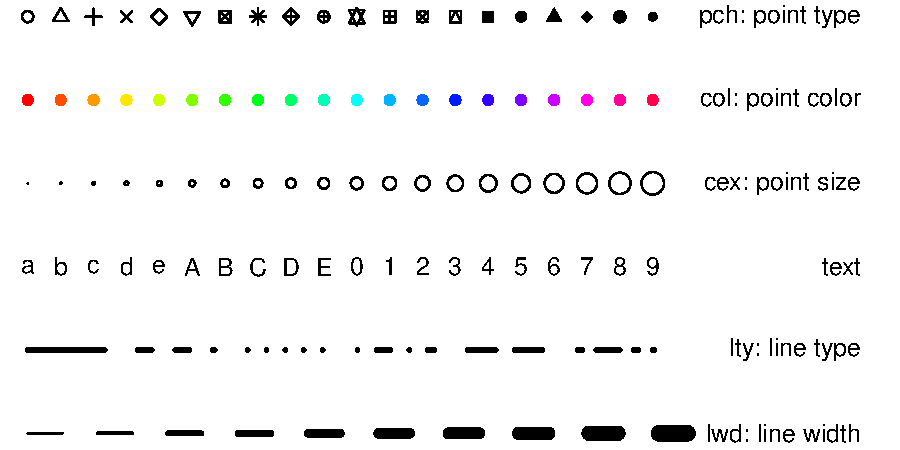
\includegraphics{lab1_files/figure-latex/unnamed-chunk-17-1.pdf}
\caption{Graphical summary of regression analysis}
\end{figure}

You can get the coefficients by using the \texttt{coef} function:

\begin{Shaded}
\begin{Highlighting}[]
\KeywordTok{coef}\NormalTok{(fit)}
\end{Highlighting}
\end{Shaded}

\begin{verbatim}
## (Intercept)       Light 
##  1.58095214  0.01361776
\end{verbatim}

You can also ``interrogate'' \texttt{fit} directly. Type
\texttt{names(fit)} to get a list of the components of \texttt{fit}, and
then use the \texttt{\$} symbol to extract components according to their
names.

\begin{Shaded}
\begin{Highlighting}[]
\KeywordTok{names}\NormalTok{(fit)}
\end{Highlighting}
\end{Shaded}

\begin{verbatim}
##  [1] "coefficients"  "residuals"     "effects"       "rank"         
##  [5] "fitted.values" "assign"        "qr"            "df.residual"  
##  [9] "xlevels"       "call"          "terms"         "model"
\end{verbatim}

For more information (perhaps more than you want) about \texttt{fit},
use \texttt{str(fit)} (for \textbf{str}ucture). You can get the
regression coefficients this way:

\begin{Shaded}
\begin{Highlighting}[]
\NormalTok{fit}\OperatorTok{$}\NormalTok{coefficients}
\end{Highlighting}
\end{Shaded}

\begin{verbatim}
## (Intercept)       Light 
##  1.58095214  0.01361776
\end{verbatim}

It's good to be able to look inside R objects when necessary, but all
other things being equal you should prefer (e.g.) \texttt{coef(x)} to
\texttt{x\$coefficients}.

\section{R interfaces}\label{r-interfaces}

\subsection{Editors and GUIs}\label{editors-and-guis}

While R works perfectly well out of the box, there are interfaces that
can make your R experience easier. Editors such as Tinn-R (Windows:
\url{http://www.sciviews.org/Tinn-R/}), Kate (Linux:
\url{http://kate-editor.org}), or Emacs/ESS (cross-platform:
\url{http://ess.r-project.org/} will color R commands and quoted
material, allow you to submit lines or blocks of R code to an R session,
and give hints about function arguments: the standard MacOS interface
has all of these features built in. Graphical interfaces such as JGR
(cross-platform: \url{http://rosuda.org/JGR/}) or SciViews (Windows:
\url{http://www.sciviews.org/SciViews-R/}) include similar editors and
have extra functions such as a workspace browser for looking at all the
variables you have defined. (All of these interfaces, which are designed
to facilitate R programming, are in a different category from Rcmdr,
which tries to simplify basic statistics in R.) If you are using Windows
or Linux I would strongly recommend that, once you have tried R a little
bit, you download at least an R-aware editor and possibly a GUI to make
your life easier. Links to all of these systems, and more, can be found
at \url{http://www.r-project.org/GUI/}.

\subsection{Script files and data
files}\label{script-files-and-data-files}

Modeling and complicated data analysis are often much easier if you use
\emph{scripts}, which are a series of commands stored in a text file.
The Windows and MacOS versions of R both have basic script editors: you
can also use Windows Notepad or Wordpad, or a more featureful editor
like PFE, Xemacs, or Tinn-R: you \textbf{should not} use MS Word.

Most programs for working with models or analyzing data follow a simple
pattern of program parts:

\begin{enumerate}
\def\labelenumi{\arabic{enumi}.}
\item
  ``Setup'' statements.
\item
  Input some data from a file or the keyboard.
\item
  Carry out the calculations that you want.
\item
  Print the results, graph them, or save them to a file.
\end{enumerate}

For example, a script file might

\begin{itemize}
\item
  Load some packages, or run another script file that creates some
  functions (more on functions later).
\item
  Read in data from a text file.
\item
  Fit several statistical models to the data and compare them.
\item
  Graph the results, and save the graph to disk for including in your
  term project.
\end{itemize}

Even for relatively simple tasks, script files are useful for building
up a calculation step-by-step, making sure that each part works before
adding on to it.

Tips for working with data and script files (sounding slightly scary but
just trying to help you avoid common pitfalls):

\begin{itemize}
\item
  To tell R where data and script files are located, you can do any one
  of the following:
\item
  spell out the \emph{path}, or file location, explicitly. (Use a single
  forward slash to separate folders (e.g.
  \texttt{"c:/My\ Documents/R/script.R"}): this works on all platforms.)
\item
  use \texttt{filename=file.choose()} (this works on all platforms, but
  is only useful on Windows and MacOS).
\item
  change your working directory to wherever the file(s) are located
  using \texttt{Change\ dir} in the \texttt{File} menu (Windows: on Mac
  it's \texttt{Misc/Change\ Working\ Directory});
\item
  change your working directory to wherever the file(s) are located
  using the \texttt{setwd} (\textbf{set} \textbf{w}orking
  \textbf{d}irectory) function, e.g. \texttt{setwd("c:/temp")}
\end{itemize}

Changing your working directory is more efficient in the long run, if
you save all the script and data files for a particular project in the
same directory and switch to that directory when you start work.

If you have a shortcut defined for R on your desktop (or in the Start
menu) you can \emph{permanently} change your default working directory
by right-clicking on the shortcut icon, selecting \texttt{Properties},
and changing the starting directory to somewhere like (for example)
\texttt{My\ Documents/R\ work}.

\begin{itemize}
\item
  it's vital that you save your data and script files as \emph{plain
  text} (or sometimes comma-separated) files. There are three things
  that can go wrong here: (1) if you use a web browser to download
  files, be careful that it doesn't automatically append some weird
  suffix to the files; (2) if your web browser has a ``file
  association'' (e.g.~it thinks that all files ending in \texttt{.dat}
  are Excel files), make sure to save the file as plain text, and
  without any extra extensions; (3) \textbf{never, (never, never) use
  Microsoft Word to edit your data and script files}; MS Word will try
  very hard to get you to save them as Word (rather than text) files,
  which will screw them up!
\item
  If you send script files by e-mail, even if you paste them into the
  message as plain text, lines will occasionally get broken in different
  places --- leading to confusion. Beware.
\end{itemize}

As a first example, the file \texttt{Intro1.R} has the commands from the
interactive regression analysis. \textbf{Important:} before working with
an example file, create a personal copy in some location on your own
computer. We will refer to this location as your \emph{temp folder}. At
the end of a lab session you \emph{must} move files onto your personal
disk (or email them to yourself).

Now open \textbf{your copy} of \texttt{Intro1.R}. In your editor, select
and Copy the entire text of the file, and then Paste the text into the R
console window (\texttt{Ctrl-C} and \texttt{Ctrl-V} as shortcuts). This
has the same effect as entering the commands by hand into the console:
they will be executed and so a graph is displayed with the results.
Cut-and-Paste allows you to execute script files one piece at a time
(which is useful for finding and fixing errors). The \texttt{source}
function allows you to run an entire script file, e.g.

\begin{Shaded}
\begin{Highlighting}[]
\KeywordTok{source}\NormalTok{(}\StringTok{"c:/temp/Intro1.R"}\NormalTok{)}
\end{Highlighting}
\end{Shaded}

You can also \texttt{source} files by pointing and clicking via the
\texttt{File} menu on the console window.

Another important time-saver is loading data from a text file. Grab
copies of \texttt{Intro2.R} and \texttt{ChlorellaGrowth.txt} from the
web page to see how this is done. In \texttt{ChlorellaGrowth.txt} the
two variables are entered as columns of a data matrix. Then instead of
typing these in by hand, the command

\begin{Shaded}
\begin{Highlighting}[]
\NormalTok{X=}\KeywordTok{read.table}\NormalTok{(}\StringTok{"ChlorellaGrowth.txt"}\NormalTok{,}\DataTypeTok{header=}\OtherTok{TRUE}\NormalTok{)}
\end{Highlighting}
\end{Shaded}

reads the file (from the current directory) and puts the data values
into the variable \texttt{X}; \texttt{header=TRUE} specifies that the
file includes column names. \textbf{Note} that as specified above you
need to make sure that R is looking for the data file in the right place
\ldots{} either move the data file to your current working directory, or
change the line so that it points to the actual location of the data
file.

Extract the variables from \texttt{X} with the commands

\begin{Shaded}
\begin{Highlighting}[]
\NormalTok{Light=X[,}\DecValTok{1}\NormalTok{]}
\NormalTok{rmax=X[,}\DecValTok{2}\NormalTok{]}
\end{Highlighting}
\end{Shaded}

Think of these as shorthand for ``\texttt{Light} = everything in column
1 of \texttt{X}'', and ``\texttt{rmax} = everything in column 2 of
\texttt{X}'' (we'll learn about working with data matrices later). From
there on out it's the same as before, with some additions that set the
axis labels and add a title.

\textbf{Exercise 5.1} Make a copy of \texttt{Intro2.R} under a new name,
and modify the copy so that it does linear regression of algal growth
rate on the natural log of light intensity,
\texttt{LogLight=log(Light)}, and plots the data appropriately. You
should end up with a graph that resembles Figure 3. (\emph{Hint:} when
you switch from light intensity to log light intensity, the range on
your \(x\) axis will change and you will have to change the \(x\)
position at which you plot the growth rate equation.)

\begin{figure}
\centering
\includegraphics{lab1_files/figure-latex/unnamed-chunk-24-1.pdf}
\caption{Graphical summary of regression analysis, using log of light
intensity (and annotating the plot)}
\end{figure}

\textbf{Exercise 5.2} Run \texttt{Intro2.R}, then enter the command
\texttt{plot(fit)} in the console and follow the directions in the
console. Figure out what just happened by entering \texttt{?plot.lm} to
bring up the Help page for the function \texttt{plot.lm} that carries
out a \texttt{plot} command for an object produced by \texttt{lm}. (This
is one example of how R uses the fact that statistical analyses are
stored as model objects. \texttt{fit} ``knows'' what kind of object it
is (in this case an object of type \texttt{lm}), and so
\texttt{plot(fit)} invokes a function that produces plots suitable for
an \texttt{lm} object.) \textbf{Answer:} R produced a series of
diagnostic plots exploring whether or not the fitted linear model is a
suitable fit to the data. In each of the plots, the 3 most extreme
points (the most likely candidates for ``outliers'') have been
identified according to their sequence in the data set.

\textbf{Exercise 5.3} The axes in plots are scaled automatically, but
the outcome is not always ideal (e.g.~if you want several graphs with
exactly the same axis limits). You can use the \texttt{xlim} and
\texttt{ylim} arguments in \texttt{plot} to control the limits:

\begin{verbatim}
plot(x,y,xlim=c(x1,x2), [other stuff]) 
\end{verbatim}

will draw the graph with the \(x\)-axis running from \texttt{x1} to
\texttt{x2}, and using \texttt{ylim=c(y1,y2)} within the \texttt{plot}
command will do the same for the \(y\)-axis.

Create a plot of growth rate versus light intensity with the \(x\)-axis
running from 0 to 120 and the \(y\)-axis running from 1 to 4.

\textbf{Exercise 5.4} You can place several graphs within a single
figure by using the \texttt{par} function (short for ``parameter'') to
adjust the layout of the plot. For example, the command

\begin{Shaded}
\begin{Highlighting}[]
\KeywordTok{par}\NormalTok{(}\DataTypeTok{mfrow=}\KeywordTok{c}\NormalTok{(}\DecValTok{2}\NormalTok{,}\DecValTok{3}\NormalTok{))}
\end{Highlighting}
\end{Shaded}

divides the plotting area into 2 rows and 3 columns. As R draws a series
of graphs, it places them along the top row from left to right, then
along the next row, and so on. \texttt{mfcol=c(2,3)} has the same effect
except that R draws successive graphs down the first column, then down
the second column, and so on.

Save \texttt{Intro2.R} with a new name and modify the program as
follows. Use \texttt{mfcol=c(2,1)} to create graphs of growth rate as a
function of \texttt{Light}, and of \texttt{log(growth\ rate)} as a
function of \texttt{log(Light)} in the same figure. Do the same again,
using \texttt{mfcol=c(1,2)}.

\textbf{Exercise 5.5 * } Use \texttt{?par} to read about other plot
control parameters that you use \texttt{par} to set (you should
definitely skim --- this is one of the longest help files in the whole R
system!). Then draw a \(2 \times 2\) set of plots, each showing the line
\(y=5x+3\) with \(x\) running from 3 to 8, but with 4 different line
styles and 4 different line colors.

\textbf{Exercise 5.6 * } Modify one of your scripts so that at the very
end it saves the plot to disk. In Windows you can do this with
\texttt{savePlot}, otherwise with \texttt{dev.print}. Use
\texttt{?savePlot}, \texttt{?dev.print} to read about these functions.
Note that the argument \texttt{filename} can include the path to a
folder; for example, in Windows you can use
\texttt{filename="c:/temp/Intro2Figure".}

(These are really exercises in using the help system, with the bonus
that you learn some things about \texttt{plot}. (Let's see, we know
\texttt{plot} can graph data points (\(r_{max}\) versus \(Light\) and
all that). Maybe it can also draw a line to connect the points, or just
draw the line and leave out the points. That would be useful. So let's
try \texttt{?plot} and see if it says anything about lines \ldots{} Hey,
it also says that
\texttt{graphical\ parameters\ can\ be\ given\ as\ arguments\ to\ plot},
so maybe I can set line colors inside the plot command instead of using
\texttt{par} all the time \ldots{}) The help system can be quite helpful
(amazingly enough) once you get used to it and get in the habit of using
it often.)

The main point is not to be afraid of experimenting; if you have saved
your previous commands in a script file, there's almost nothing you can
break by trying out commands and inspecting the results.

\section{The R package system}\label{the-r-package-system}

R has many extra packages that provide extra functions. You may be able
to install new packages from a menu within R. You can always type

\begin{Shaded}
\begin{Highlighting}[]
\KeywordTok{install.packages}\NormalTok{(}\StringTok{"plotrix"}\NormalTok{)}
\end{Highlighting}
\end{Shaded}

(for example --- this installs the \texttt{plotrix} package). You can
install more than one package at a time:

\begin{Shaded}
\begin{Highlighting}[]
\KeywordTok{install.packages}\NormalTok{(}\KeywordTok{c}\NormalTok{(}\StringTok{"ellipse"}\NormalTok{,}\StringTok{"plotrix"}\NormalTok{))}
\end{Highlighting}
\end{Shaded}

(\texttt{c} stands for ``combine'', and is the command for combining
multiple things into a single object.) If the machine on which you use R
is not connected to the Internet, you can download the packages to some
other medium (such as a flash drive or CD) and install them later, using
\texttt{Install\ from\ local\ zip\ file} in the menu or

\begin{Shaded}
\begin{Highlighting}[]
\KeywordTok{install.packages}\NormalTok{(}\StringTok{"plotrix"}\NormalTok{,}\DataTypeTok{repos=}\OtherTok{NULL}\NormalTok{)}
\end{Highlighting}
\end{Shaded}

If you do not have permission to install packages in R's central
directory, R will may ask whether you want to install the packages in a
user-specific directory.

If you install the \texttt{emdbook} package first
(\texttt{install.packages("emdbook")}), load the package
(\texttt{library(emdbook)}), and then run the command
\texttt{get.emdbook.packages()} (you do need the empty parentheses) it
will install these packages for you automatically.

(\texttt{R2WinBUGS} is an exception to R's normally seamless
cross-platform operation: it depends on a Windows program called
WinBUGS. WinBUGS will also run on Linux or MacOS {[}on Intel
hardware{]}, with the help of a program called WINE (we'll deal with
this later).)

It will save time if you install these packages now.

\section{Statistics in R}\label{statistics-in-r}

Some of the important functions and packages (collections of functions)
for statistical modeling and data analysis are summarized in Table 2.
Venables and Ripley (2002) give a good practical (although somewhat
advanced) overview, and you can find a list of available packages and
their contents at CRAN, the main R website
(\url{http://www.cran.r-project.org} --- select a mirror site near you
and click on \texttt{Package\ sources}). For the most part, we will not
be concerned here with this side of R.

\begin{table}

\caption{\label{tab:unnamed-chunk-29}A few of the functions and packages in R for statistical modeling and data analysis. There are \emph{many} more, but you will have to learn about them somewhere else.}
\centering
\resizebox{\linewidth}{!}{
\begin{tabular}[t]{ll}
\toprule
Function & Definition and packages\\
\midrule
\texttt{aov}, \texttt{anova} & Analysis of variance or deviance\\
\texttt{lm} & Linear models (regression, ANOVA, ANCOVA)\\
\texttt{glm} & Generalized linear models (e.g. logistic, Poisson regression)\\
\texttt{gam} & Generalized additive models (in package \texttt{mgcv})\\
\texttt{nls} & Fit nonlinear models by least-squares\\
\addlinespace
\texttt{lme}, \texttt{nlme},\texttt{lmer}, \texttt{glmer} & Linear, generalized linear, and nonlinear mixed-effects models\\
 & (repeated measures, block effects, spatial models) in packages\\
 & \texttt{nlme} and \texttt{lme4}\\
\texttt{boot} & Package: bootstrapping functions\\
\texttt{splines} & Package: nonparametric regression (more in packages \texttt{fields},\\
\addlinespace
 & \texttt{KernSmooth}, \texttt{logspline}, \texttt{sm} and others)\\
\texttt{princomp}, \texttt{manova}, \texttt{lda}, \texttt{cancor} & Multivariate analysis (some in package \texttt{MASS}; also see packages\\
 & \texttt{vegan}, \texttt{ade4})\\
\texttt{survival} & Package: survival analysis\\
\texttt{tree}, \texttt{rpart} & Packages: tree-based regression\\
\bottomrule
\end{tabular}}
\end{table}

\section{Vectors}\label{vectors}

Vectors and matrices (1- and 2-dimensional rectangular arrays of
numbers) are pre-defined data types in R. Operations with vectors and
matrices may seem a bit abstract now, but we need them to do useful
things later. Vectors' only properties are their type (or \emph{class})
and length, although they can also have an associated list of names.

We've already seen two ways to create vectors in R:

\begin{enumerate}
\def\labelenumi{\arabic{enumi}.}
\tightlist
\item
  A command in the console window or a script file listing the values,
  such as
\end{enumerate}

\begin{Shaded}
\begin{Highlighting}[]
\NormalTok{initialsize=}\KeywordTok{c}\NormalTok{(}\DecValTok{1}\NormalTok{,}\DecValTok{3}\NormalTok{,}\DecValTok{5}\NormalTok{,}\DecValTok{7}\NormalTok{,}\DecValTok{9}\NormalTok{,}\DecValTok{11}\NormalTok{)}
\end{Highlighting}
\end{Shaded}

\begin{enumerate}
\def\labelenumi{\arabic{enumi}.}
\setcounter{enumi}{1}
\tightlist
\item
  Using \texttt{read.table}:
\end{enumerate}

\begin{Shaded}
\begin{Highlighting}[]
\NormalTok{initialsize=}\KeywordTok{read.table}\NormalTok{(}\StringTok{"c:/temp/initialdata.txt"}\NormalTok{)}
\end{Highlighting}
\end{Shaded}

(assuming of course that the file exists in the right place).

You can then use a vector in calculations as if it were a number (more
or less)

\begin{Shaded}
\begin{Highlighting}[]
\NormalTok{finalsize=initialsize}\OperatorTok{+}\DecValTok{1}
\NormalTok{newsize=}\KeywordTok{sqrt}\NormalTok{(initialsize)}
\NormalTok{finalsize}
\end{Highlighting}
\end{Shaded}

\begin{verbatim}
## [1]  2  4  6  8 10 12
\end{verbatim}

Notice that R applied each operation to every entry in the vector.
Similarly, commands like
\texttt{initialsize-5,\ 2*initialsize,\ initialsize/10} apply
subtraction, multiplication, and division to each element of the vector.
The same is true for

\begin{Shaded}
\begin{Highlighting}[]
\NormalTok{initialsize}\OperatorTok{^}\DecValTok{2}
\end{Highlighting}
\end{Shaded}

\begin{verbatim}
## [1]   1   9  25  49  81 121
\end{verbatim}

In R the default is to apply functions and operations to vectors in an
\emph{element by element} (or ``vectorized'') manner.

\subsection{Functions for creating
vectors}\label{functions-for-creating-vectors}

You can use the \texttt{seq} function to create a set of regularly
spaced values. \texttt{seq}'s syntax is \texttt{x=seq(from,to,by)} or
\texttt{x=seq(from,to)} or \texttt{x=seq(from,to,length.out)}

The first form generates a vector \texttt{(from,from+by,from+2*by,...)}
with the last entry not extending further than than \texttt{to}. In the
second form the value of \texttt{by} is assumed to be 1 or -1, depending
on whether \texttt{from} or \texttt{to} is larger. The third form
creates a vector with the desired endpoints and length. The syntax
\texttt{from:to} is a shortcut for \texttt{seq(from,to)}:

\begin{Shaded}
\begin{Highlighting}[]
\DecValTok{1}\OperatorTok{:}\DecValTok{8}
\end{Highlighting}
\end{Shaded}

\begin{verbatim}
## [1] 1 2 3 4 5 6 7 8
\end{verbatim}

\textbf{Exercise 8.1} Use \texttt{seq} to create the vector
\texttt{v=(1\ 5\ 9\ 13)}, and to create a vector going from 1 to 5 in
increments of 0.2.

You can use \texttt{rep} to create a constant vector such as
\texttt{(1\ 1\ 1\ 1)}; the basic syntax is \texttt{rep(values,lengths)}.
For example,

\begin{Shaded}
\begin{Highlighting}[]
\KeywordTok{rep}\NormalTok{(}\DecValTok{3}\NormalTok{,}\DecValTok{5}\NormalTok{)}
\end{Highlighting}
\end{Shaded}

\begin{verbatim}
## [1] 3 3 3 3 3
\end{verbatim}

creates a vector in which the value 3 is repeated 5 times. \texttt{rep}
will repeat a whole vector multiple times

\begin{Shaded}
\begin{Highlighting}[]
\KeywordTok{rep}\NormalTok{(}\DecValTok{1}\OperatorTok{:}\DecValTok{3}\NormalTok{,}\DecValTok{3}\NormalTok{)}
\end{Highlighting}
\end{Shaded}

\begin{verbatim}
## [1] 1 2 3 1 2 3 1 2 3
\end{verbatim}

or will repeat each of the elements in a vector a given number of times:

\begin{Shaded}
\begin{Highlighting}[]
\KeywordTok{rep}\NormalTok{(}\DecValTok{1}\OperatorTok{:}\DecValTok{3}\NormalTok{,}\DataTypeTok{each=}\DecValTok{3}\NormalTok{)}
\end{Highlighting}
\end{Shaded}

\begin{verbatim}
## [1] 1 1 1 2 2 2 3 3 3
\end{verbatim}

Even more flexibly, you can repeat each element in the vector a
different number of times:

\begin{Shaded}
\begin{Highlighting}[]
\KeywordTok{rep}\NormalTok{( }\KeywordTok{c}\NormalTok{(}\DecValTok{3}\NormalTok{,}\DecValTok{4}\NormalTok{),}\KeywordTok{c}\NormalTok{(}\DecValTok{2}\NormalTok{,}\DecValTok{5}\NormalTok{) )}
\end{Highlighting}
\end{Shaded}

\begin{verbatim}
## [1] 3 3 4 4 4 4 4
\end{verbatim}

The value 3 was repeated 2 times, followed by the value 4 repeated 5
times. \texttt{rep} can be a little bit mind-blowing as you get started,
but it will turn out to be useful.

Table 3 lists some of the main functions for creating and working with
vectors.

\begin{table}

\caption{\label{tab:unnamed-chunk-39}Some important R functions for creating and working with vectors. Many of these have other optional arguments; use the help system (e.g. \texttt{?cor}) for more information. The statistical functions such as \texttt{var} regard the values as samples from a population and compute an estimate of the population statistic; for example \texttt{sd(1:3)=1}.}
\centering
\resizebox{\linewidth}{!}{
\begin{tabular}[t]{ll}
\toprule
Function & Definition\\
\midrule
\texttt{seq(from,to,by=1)} & Vector of evenly spaced values, default increment = 1)\\
\texttt{seq(from, to, length.out)} & Vector of evenly spaced values, specified length)\\
\texttt{c(u,v,...)} & Combine a set of numbers and/or vectors into a single vector\\
\texttt{rep(a,b)} & Create vector by repeating elements of \texttt{a} by amounts in \texttt{b}\\
\texttt{as.vector(x)} & Convert an object of some other type to a vector\\
\addlinespace
\texttt{hist(v)} & Histogram plot of value in v\\
\texttt{mean(v),var(v),sd(v)} & Estimate of population mean, variance, standard deviation\\
 & based on data values in \texttt{v}\\
\texttt{cor(v,w)} & Correlation between two vectors\\
\bottomrule
\end{tabular}}
\end{table}

\subsection{Vector indexing}\label{vector-indexing}

You will often want to extract a specific entry or other part of a
vector. This procedure is called \emph{vector indexing}, and uses square
brackets (\texttt{{[}{]}}):

\begin{Shaded}
\begin{Highlighting}[]
\NormalTok{z=}\KeywordTok{c}\NormalTok{(}\DecValTok{1}\NormalTok{,}\DecValTok{3}\NormalTok{,}\DecValTok{5}\NormalTok{,}\DecValTok{7}\NormalTok{,}\DecValTok{9}\NormalTok{,}\DecValTok{11}\NormalTok{)}
\NormalTok{z[}\DecValTok{3}\NormalTok{]}
\end{Highlighting}
\end{Shaded}

\begin{verbatim}
## [1] 5
\end{verbatim}

(how would you use \texttt{seq} to construct \texttt{z}?)
\texttt{z{[}3{]}} extracts the third item, or \emph{element}, in the
vector \texttt{z}. You can also access a block of elements using the
functions for vector construction, e.g.

\begin{Shaded}
\begin{Highlighting}[]
\NormalTok{z[}\DecValTok{2}\OperatorTok{:}\DecValTok{5}\NormalTok{]}
\end{Highlighting}
\end{Shaded}

\begin{verbatim}
## [1] 3 5 7 9
\end{verbatim}

extracts the second through fifth elements.

What happens if you enter \texttt{v=z{[}seq(1,5,2){]}} ? Try it and see,
and make sure you understand what happened.

You can extracted irregularly spaced elements of a vector. For example

\begin{Shaded}
\begin{Highlighting}[]
\NormalTok{z[}\KeywordTok{c}\NormalTok{(}\DecValTok{1}\NormalTok{,}\DecValTok{2}\NormalTok{,}\DecValTok{5}\NormalTok{)]}
\end{Highlighting}
\end{Shaded}

\begin{verbatim}
## [1] 1 3 9
\end{verbatim}

You can also use indexing to \textbf{set specific values within a
vector}. For example,

\begin{Shaded}
\begin{Highlighting}[]
\NormalTok{z[}\DecValTok{1}\NormalTok{]=}\DecValTok{12}
\end{Highlighting}
\end{Shaded}

changes the value of the first entry in \texttt{z} while leaving all the
rest alone, and

\begin{Shaded}
\begin{Highlighting}[]
\NormalTok{z[}\KeywordTok{c}\NormalTok{(}\DecValTok{1}\NormalTok{,}\DecValTok{3}\NormalTok{,}\DecValTok{5}\NormalTok{)]=}\KeywordTok{c}\NormalTok{(}\DecValTok{22}\NormalTok{,}\DecValTok{33}\NormalTok{,}\DecValTok{44}\NormalTok{)}
\end{Highlighting}
\end{Shaded}

changes the first, third, and fifth values (note that we had to use
\texttt{c} to create the vector --- can you interpret the error message
you get if you try \texttt{z{[}1,3,5{]}} ?)

\textbf{Exercise 8.2} Write a \emph{one-line} command to extract a
vector consisting of the second, first, and third elements of \texttt{z}
\emph{in that order}.

\textbf{Exercise 8.3} Write a script file that computes values of
\(y=\frac{(x-1)}{(x+1)}\) for \(x=1,2,\cdots,10\), and plots \(y\)
versus \(x\) with the points plotted and connected by a line (hint: in
\texttt{?plot}, search for \texttt{type}).

\textbf{Exercise 8.4* } The sum of the geometric series
\(1 + r + r^2 + r^3 + ... + r^n\) approaches the limit \(1/(1-r)\) for
\(r < 1\) as \(n \rightarrow \infty\). Set the values \(r=0.5\) and
\(n=10\), and then write a \textbf{one-line} command that creates the
vector \(G = (r^0,r^1,r^2,...,r^n)\). Compare the sum (using
\texttt{sum}) of this vector to the limiting value \(1/(1-r)\). Repeat
for \(n=50\). (\emph{Note} that comparing very similar numeric values
can be tricky: rounding can happen, and some numbers cannot be
represented exactly in binary (computer) notation. By default R displays
7\textasciitilde{}significant digits (\texttt{options("digits")}).

For example:

\begin{Shaded}
\begin{Highlighting}[]
\NormalTok{x =}\StringTok{ }\FloatTok{1.999999}
\NormalTok{x}
\end{Highlighting}
\end{Shaded}

\begin{verbatim}
## [1] 1.999999
\end{verbatim}

\begin{Shaded}
\begin{Highlighting}[]
\NormalTok{x}\OperatorTok{-}\DecValTok{2}
\end{Highlighting}
\end{Shaded}

\begin{verbatim}
## [1] -1e-06
\end{verbatim}

\begin{Shaded}
\begin{Highlighting}[]
\NormalTok{x=}\FloatTok{1.9999999999999}
\NormalTok{x}
\end{Highlighting}
\end{Shaded}

\begin{verbatim}
## [1] 2
\end{verbatim}

\begin{Shaded}
\begin{Highlighting}[]
\NormalTok{x}\OperatorTok{-}\DecValTok{2}
\end{Highlighting}
\end{Shaded}

\begin{verbatim}
## [1] -9.992007e-14
\end{verbatim}

All the digits are still there, in the second case, but they are not
shown. Also note that \texttt{x-2} is not exactly
\(-1 \times 10^{-13}\); this is unavoidable.)

\subsection{Logical operators}\label{logical-operators}

Logical operators return a value of \texttt{TRUE} or \texttt{FALSE}. For
example, try:

\begin{Shaded}
\begin{Highlighting}[]
\NormalTok{a=}\DecValTok{1}
\NormalTok{b=}\DecValTok{3}
\NormalTok{c=a}\OperatorTok{<}\NormalTok{b}
\NormalTok{d=(a}\OperatorTok{>}\NormalTok{b)}
\NormalTok{c}
\end{Highlighting}
\end{Shaded}

\begin{verbatim}
## [1] TRUE
\end{verbatim}

\begin{Shaded}
\begin{Highlighting}[]
\NormalTok{d}
\end{Highlighting}
\end{Shaded}

\begin{verbatim}
## [1] FALSE
\end{verbatim}

The parentheses around (\texttt{a\textgreater{}b}) are optional but make
the code easier to read. One special case where you \emph{do} need
parentheses (or spaces) is when you make comparisons with negative
values; \texttt{a\textless{}-1} will surprise you by setting
\texttt{a=1}, because \texttt{\textless{}-} (representing a
left-pointing arrow) is equivalent to \texttt{=} in R. Use
\texttt{a\textless{}\ -1}, or more safely \texttt{a\textless{}(-1)}, to
make this comparison.

\begin{table}

\caption{\label{tab:unnamed-chunk-47}Some comparison operators in R. Use \texttt{?Comparison} to learn more.}
\centering
\begin{tabular}[t]{ll}
\toprule
Operator & Definition\\
\midrule
\texttt{x<y} & less than\\
\texttt{x>y} & greater than\\
\texttt{x<=y} & less than or equal to\\
\texttt{x>=y} & greater than or equal to\\
\texttt{x==y} & equal to\\
\texttt{x!=y} & \emph{not} equal to\\
\bottomrule
\end{tabular}
\end{table}

When we compare two vectors or matrices of the same size, or compare a
number with a vector or matrix, comparisons are done element-by-element.
For example,

\begin{Shaded}
\begin{Highlighting}[]
\NormalTok{x=}\DecValTok{1}\OperatorTok{:}\DecValTok{5}
\NormalTok{(}\DataTypeTok{b=}\NormalTok{(x}\OperatorTok{<=}\DecValTok{3}\NormalTok{))}
\end{Highlighting}
\end{Shaded}

\begin{verbatim}
## [1]  TRUE  TRUE  TRUE FALSE FALSE
\end{verbatim}

So if \texttt{x} and \texttt{y} are vectors, then \texttt{(x==y)} will
return a vector of values giving the element-by-element comparisons. If
you want to know whether \texttt{x} and \texttt{y} are identical
vectors, use \texttt{identical(x,y)} which returns a single value:
\texttt{TRUE} if each entry in \texttt{x} equals the corresponding entry
in \texttt{y}, otherwise \texttt{FALSE}. You can use \texttt{?Logical}
to read more about logical operators. \textbf{Note the difference
between = and ==: can you figure out what happened in the following
cautionary tale?}

\begin{Shaded}
\begin{Highlighting}[]
\NormalTok{a =}\StringTok{ }\DecValTok{1}\OperatorTok{:}\DecValTok{3}
\NormalTok{b =}\StringTok{ }\DecValTok{2}\OperatorTok{:}\DecValTok{4}
\NormalTok{a}\OperatorTok{==}\NormalTok{b}
\end{Highlighting}
\end{Shaded}

\begin{verbatim}
## [1] FALSE FALSE FALSE
\end{verbatim}

\begin{Shaded}
\begin{Highlighting}[]
\NormalTok{a=b}
\NormalTok{a}\OperatorTok{==}\NormalTok{b}
\end{Highlighting}
\end{Shaded}

\begin{verbatim}
## [1] TRUE TRUE TRUE
\end{verbatim}

Exclamation points \texttt{!} are used in R to mean ``not''; \texttt{!=}
(not \texttt{==}) means ``not equal to''.

R also does arithmetic on logical values, treating \texttt{TRUE} as 1
and \texttt{FALSE} as 0. So \texttt{sum(b)} returns the value 3, telling
us that three entries of \texttt{x} satisfied the condition
(\texttt{x\textless{}=3}). This is useful for (e.g.) seeing how many of
the elements of a vector are larger than a cutoff value.

Build more complicated conditions by using \emph{logical operators} to
combine comparisons:

\begin{itemize}
\tightlist
\item
  \texttt{!}: Negation
\item
  \texttt{\&}, \texttt{\&\&}: AND
\item
  \texttt{\textbar{}}, \texttt{\textbar{}\textbar{}}: O
\end{itemize}

OR is \emph{non-exclusive}, meaning that \texttt{x\textbar{}y} is true
if either \texttt{x} or \texttt{y} \emph{or both} are true (a
ham-and-cheese sandwich would satisfy the condition ``ham OR cheese'').
For example, try

\begin{Shaded}
\begin{Highlighting}[]
\NormalTok{a=}\KeywordTok{c}\NormalTok{(}\DecValTok{1}\NormalTok{,}\DecValTok{2}\NormalTok{,}\DecValTok{3}\NormalTok{,}\DecValTok{4}\NormalTok{)}
\NormalTok{b=}\KeywordTok{c}\NormalTok{(}\DecValTok{1}\NormalTok{,}\DecValTok{1}\NormalTok{,}\DecValTok{5}\NormalTok{,}\DecValTok{5}\NormalTok{)}
\NormalTok{(a}\OperatorTok{<}\NormalTok{b)}\OperatorTok{&}\StringTok{ }\NormalTok{(a}\OperatorTok{>}\DecValTok{3}\NormalTok{)}
\end{Highlighting}
\end{Shaded}

\begin{verbatim}
## [1] FALSE FALSE FALSE  TRUE
\end{verbatim}

\begin{Shaded}
\begin{Highlighting}[]
\NormalTok{(a}\OperatorTok{<}\NormalTok{b) }\OperatorTok{|}\StringTok{ }\NormalTok{(a}\OperatorTok{>}\DecValTok{3}\NormalTok{)}
\end{Highlighting}
\end{Shaded}

\begin{verbatim}
## [1] FALSE FALSE  TRUE  TRUE
\end{verbatim}

and make sure you understand what happened (if it's confusing, try
breaking up the expression and looking at the results of
\texttt{a\textless{}b} and \texttt{a\textgreater{}3} separately first).
The two forms of AND and OR differ in how they handle vectors. The
shorter one does element-by-element comparisons; the longer one only
looks at the first element in each vector.

\subsection{Vector indexing II}\label{vector-indexing-ii}

We can also use \emph{logical} vectors (lists of \texttt{TRUE} and
\texttt{FALSE} values) to pick elements out of vectors. This is
important, e.g., for subsetting data (getting rid of those pesky
outliers!)

As a simple example, we might want to focus on just the low-light values
of \(r_{max}\) in the \emph{Chlorella} example:

\begin{Shaded}
\begin{Highlighting}[]
\NormalTok{X=}\KeywordTok{read.table}\NormalTok{(}\StringTok{"ChlorellaGrowth.txt"}\NormalTok{,}\DataTypeTok{header=}\OtherTok{TRUE}\NormalTok{)}
\NormalTok{Light=X[,}\DecValTok{1}\NormalTok{]}
\NormalTok{rmax=X[,}\DecValTok{2}\NormalTok{]}
\NormalTok{lowLight =}\StringTok{ }\NormalTok{Light[Light}\OperatorTok{<}\DecValTok{50}\NormalTok{]}
\NormalTok{lowLightrmax =}\StringTok{ }\NormalTok{rmax[Light}\OperatorTok{<}\DecValTok{50}\NormalTok{]}
\NormalTok{lowLight}
\end{Highlighting}
\end{Shaded}

\begin{verbatim}
## [1] 20 20 20 21 24 44
\end{verbatim}

\begin{Shaded}
\begin{Highlighting}[]
\NormalTok{lowLightrmax}
\end{Highlighting}
\end{Shaded}

\begin{verbatim}
## [1] 1.65 2.02 1.89 2.61 1.36 2.37
\end{verbatim}

What is really happening here (think about it for a minute) is that
\texttt{Light\textless{}50} generates a logical vector the same length
as \texttt{Light} (\texttt{TRUE\ TRUE\ TRUE\ ...}) which is then used to
select the appropriate values.

If you want the positions at which \texttt{Light} is lower than 50, you
could say \texttt{(1:length(Light)){[}Light\textless{}50{]}}, but you
can also use a built-in function: \texttt{which(Light\textless{}50)}. If
you wanted the position at which the maximum value of \texttt{Light}
occurs, you could say \texttt{which(Light==max(Light))}. (This normally
results in a vector of length 1; when could it give a longer vector?)
There is even a built-in command for this specific function,
\texttt{which.max} (although \texttt{which.max} always returns just the
\emph{first} position at which the maximum occurs).

\textbf{Exercise 8.5}: What would happen if instead of setting
\texttt{lowLight} you replaced \texttt{Light} by saying
\texttt{Light=Light{[}Light\textless{}50{]}}, and then
\texttt{rmax=rmax{[}Light\textless{}50{]}}? Why would that be wrong? Try
it with some temporary variables --- set \texttt{Light2=Light} and
\texttt{rmax2=rmax} and then play with \texttt{Light2} and
\texttt{rmax2} so you don't mess up your working variables --- and work
out what happened \ldots{}

We can also combine logical operators (making sure to use the
element-by-element \texttt{\&} and \texttt{\textbar{}} versions of AND
and OR):

\begin{Shaded}
\begin{Highlighting}[]
\NormalTok{Light[Light}\OperatorTok{<}\DecValTok{50} \OperatorTok{&}\StringTok{ }\NormalTok{rmax }\OperatorTok{<=}\StringTok{ }\FloatTok{2.0}\NormalTok{]}
\end{Highlighting}
\end{Shaded}

\begin{verbatim}
## [1] 20 20 24
\end{verbatim}

\begin{Shaded}
\begin{Highlighting}[]
\NormalTok{rmax[Light}\OperatorTok{<}\DecValTok{50} \OperatorTok{&}\StringTok{ }\NormalTok{rmax }\OperatorTok{<=}\StringTok{ }\FloatTok{2.0}\NormalTok{]}
\end{Highlighting}
\end{Shaded}

\begin{verbatim}
## [1] 1.65 1.89 1.36
\end{verbatim}

\textbf{Exercise 8.6} \texttt{runif(n)} is a function (more on it soon)
that generates a vector of \texttt{n} random, uniformly distributed
numbers between 0 and 1. Create a vector of 20 numbers, then select the
subset of those numbers that is less than the mean. (If you want your
answers to match mine exactly, use \texttt{set.seed(273)} to set the
random-number generator to a particular starting point before you use
\texttt{runif}; {[}273 is an arbitrary number I chose{]}.)

\textbf{Exercise 8.7* } Find the \emph{positions} of the elements that
are less than the mean of the vector you just created (e.g.~if your
vector were \texttt{(0.1\ 0.9.\ 0.7\ 0.3)} the answer would be
\texttt{(1\ 4)}).

As I mentioned in passing above, vectors can have names associated with
their elements: if they do, you can also extract elements by name (use
\texttt{names} to find out the names).

\begin{Shaded}
\begin{Highlighting}[]
\NormalTok{x =}\StringTok{ }\KeywordTok{c}\NormalTok{(}\DataTypeTok{first=}\DecValTok{7}\NormalTok{,}\DataTypeTok{second=}\DecValTok{5}\NormalTok{,}\DataTypeTok{third=}\DecValTok{2}\NormalTok{)}
\KeywordTok{names}\NormalTok{(x)}
\end{Highlighting}
\end{Shaded}

\begin{verbatim}
## [1] "first"  "second" "third"
\end{verbatim}

\begin{Shaded}
\begin{Highlighting}[]
\NormalTok{x[}\StringTok{"first"}\NormalTok{]}
\end{Highlighting}
\end{Shaded}

\begin{verbatim}
## first 
##     7
\end{verbatim}

\begin{Shaded}
\begin{Highlighting}[]
\NormalTok{x[}\KeywordTok{c}\NormalTok{(}\StringTok{"third"}\NormalTok{,}\StringTok{"first"}\NormalTok{)]}
\end{Highlighting}
\end{Shaded}

\begin{verbatim}
## third first 
##     2     7
\end{verbatim}

Finally, it is sometimes handy to be able to drop a particular set of
elements, rather than taking a particular set: you can do this with
negative indices. For example, \texttt{x{[}-1{]}} extracts all but the
first element of a vector.

\textbf{Exercise 8.8* }: Specify two ways to take only the elements in
the odd positions (first, third, \ldots{}) of a vector of arbitrary
length.

\section{Matrices}\label{matrices}

\subsection{Creating matrices}\label{creating-matrices}

Like vectors, you can create matrices by using \texttt{read.table} to
read in values from a data file. (Actually, this creates a data frame,
which is \emph{almost} the same as a matrix --- see section 10.2.) You
can also create matrices of numbers by creating a vector of the matrix
entries, and then reshaping them to the desired number of rows and
columns using the function \texttt{matrix}. For example

\begin{Shaded}
\begin{Highlighting}[]
\NormalTok{(}\DataTypeTok{X=}\KeywordTok{matrix}\NormalTok{(}\DecValTok{1}\OperatorTok{:}\DecValTok{6}\NormalTok{,}\DataTypeTok{nrow=}\DecValTok{2}\NormalTok{,}\DataTypeTok{ncol=}\DecValTok{3}\NormalTok{))}
\end{Highlighting}
\end{Shaded}

\begin{verbatim}
##      [,1] [,2] [,3]
## [1,]    1    3    5
## [2,]    2    4    6
\end{verbatim}

takes the values 1 to 6 and reshapes them into a 2 by 3 matrix.

By default R loads the values into the matrix \emph{column-wise} (this
is probably counter-intuitive since we're used to reading tables
row-wise). Use the optional parameter \texttt{byrow} to change this
behavior. For example :

\begin{Shaded}
\begin{Highlighting}[]
\NormalTok{(}\DataTypeTok{A=}\KeywordTok{matrix}\NormalTok{(}\DecValTok{1}\OperatorTok{:}\DecValTok{9}\NormalTok{,}\DataTypeTok{nrow=}\DecValTok{3}\NormalTok{,}\DataTypeTok{ncol=}\DecValTok{3}\NormalTok{,}\DataTypeTok{byrow=}\OtherTok{TRUE}\NormalTok{))}
\end{Highlighting}
\end{Shaded}

\begin{verbatim}
##      [,1] [,2] [,3]
## [1,]    1    2    3
## [2,]    4    5    6
## [3,]    7    8    9
\end{verbatim}

R will re-cycle through entries in the data vector, if necessary to fill
a matrix of the specified size. So for example

\begin{Shaded}
\begin{Highlighting}[]
\KeywordTok{matrix}\NormalTok{(}\DecValTok{1}\NormalTok{,}\DataTypeTok{nrow=}\DecValTok{10}\NormalTok{,}\DataTypeTok{ncol=}\DecValTok{10}\NormalTok{)}
\end{Highlighting}
\end{Shaded}

creates a \(10 \times 10\) matrix of ones.

\textbf{Exercise 9.1} Use a command of the form
\texttt{X=matrix(v,nrow=2,ncol=4)} where \texttt{v} is a data vector, to
create the following matrix \texttt{X}:

\begin{verbatim}
##      [,1] [,2] [,3] [,4]
## [1,]    1    1    1    1
## [2,]    2    2    2    2
\end{verbatim}

If you can, try to use R commands to construct the vector rather than
typing out all of the individual values.

R will also collapse a matrix to behave like a vector whenever it makes
sense: for example \texttt{sum(X)} above is 12.

\textbf{Exercise 9.2} Use \texttt{rnorm} (which is like \texttt{runif},
but generates Gaussian (normally distributed) numbers with a specified
mean and standard deviation instead) and \texttt{matrix} to create a
\(5 \times 7\) matrix of Gaussian random numbers with mean 1 and
standard deviation 2. (Use \texttt{set.seed(273)} again for
consistency.)

Another useful function for creating matrices is \texttt{diag}.
\texttt{diag(v,n)} creates an \(n \times n\) matrix with data vector
\(v\) on its diagonal. So for example \texttt{diag(1,5)} creates the
\(5 \times 5\) \emph{identity matrix}, which has 1's on the diagonal and
0 everywhere else. Try \texttt{diag(1:5,5)} and \texttt{diag(1:2,5)};
why does the latter produce a warning?

Finally, you can use the \texttt{data.entry} function. This function can
only edit existing matrices, but for example (try this now!!)

\begin{Shaded}
\begin{Highlighting}[]
\NormalTok{A=}\KeywordTok{matrix}\NormalTok{(}\DecValTok{0}\NormalTok{,}\DataTypeTok{nrow=}\DecValTok{3}\NormalTok{,}\DataTypeTok{ncol=}\DecValTok{4}\NormalTok{)}
\KeywordTok{data.entry}\NormalTok{(A)}
\end{Highlighting}
\end{Shaded}

will create \texttt{A} as a \(3 \times 4\) matrix, and then call up a
spreadsheet-like interface in which you can change the values to
whatever you need.

\begin{table}

\caption{\label{tab:unnamed-chunk-59}Some important functions for creating and working with matrices. Many of these have additional optional arguments; use the help system for full details.}
\centering
\resizebox{\linewidth}{!}{
\begin{tabular}[t]{ll}
\toprule
Function & Definition\\
\midrule
\texttt{matrix(v,nrow=m,ncol=n)} & $m \times n$ matrix using the values in \texttt{v}\\
\texttt{t(A)} & transpose (exchange rows and columns) of matrix \texttt{A}\\
\texttt{dim(X)} & dimensions of matrix X. \texttt{dim(X)[1]} = number of rows,\\
 & \texttt{dim(X)[2]} = number of columns\\
\texttt{data.entry(A)} & call up a spreadsheet-like interface to edit the values in \texttt{A}\\
\addlinespace
\texttt{diag(v,n)} & diagonal $n \times n$ matrix with $v$ on diagonal, 0 elsewhere 
(\texttt{v} is 1 by default,\\
 & so \texttt{diag(n)} gives an $n \times n$ identity matrix)\\
\texttt{cbind(a,b,c,...)} & combine compatible objects by attaching them along columns\\
\texttt{rbind(a,b,c,...)} & combine compatible objects by attaching them along rows\\
\texttt{as.matrix(x)} & convert an object of some other type to a matrix, if possible\\
\texttt{outer(v,w)} & "outer product" of vectors \texttt{v}, \texttt{w}: the matrix whose $(i,j)$th element is \texttt{v[i]*w[j]}\\
\bottomrule
\end{tabular}}
\end{table}

\subsection{\texorpdfstring{\texttt{cbind} and
\texttt{rbind}}{cbind and rbind}}\label{cbind-and-rbind}

If their sizes match, you can combine vectors to form matrices, and
stick matrices together with vectors or other matrices. \texttt{cbind}
(``column bind'') and \texttt{rbind} (``row bind'') are the functions to
use.

\texttt{cbind} binds together columns of two objects. One thing it can
do is put vectors together to form a matrix:

\begin{Shaded}
\begin{Highlighting}[]
\NormalTok{(}\DataTypeTok{C=}\KeywordTok{cbind}\NormalTok{(}\DecValTok{1}\OperatorTok{:}\DecValTok{3}\NormalTok{,}\DecValTok{4}\OperatorTok{:}\DecValTok{6}\NormalTok{,}\DecValTok{5}\OperatorTok{:}\DecValTok{7}\NormalTok{))}
\end{Highlighting}
\end{Shaded}

\begin{verbatim}
##      [,1] [,2] [,3]
## [1,]    1    4    5
## [2,]    2    5    6
## [3,]    3    6    7
\end{verbatim}

R interprets vectors as row or column vectors according to what you're
doing with them. Here it treats them as column vectors so that columns
exist to be bound together. On the other hand,

\begin{Shaded}
\begin{Highlighting}[]
\NormalTok{(}\DataTypeTok{D=}\KeywordTok{rbind}\NormalTok{(}\DecValTok{1}\OperatorTok{:}\DecValTok{3}\NormalTok{,}\DecValTok{4}\OperatorTok{:}\DecValTok{6}\NormalTok{))}
\end{Highlighting}
\end{Shaded}

\begin{verbatim}
##      [,1] [,2] [,3]
## [1,]    1    2    3
## [2,]    4    5    6
\end{verbatim}

treats them as rows. Now we have two matrices that can be combined.

\textbf{Exercise 9.3} Verify that \texttt{rbind(C,D)} works,
\texttt{cbind(C,C)} works, but \texttt{cbind(C,D)} doesn't. Why not?

\subsection{Matrix indexing}\label{matrix-indexing}

Matrix indexing is like vector indexing except that you have to specify
both the row and column, or range of rows and columns. For example
\texttt{z=A{[}2,3{]}} sets \texttt{z} equal to 6, which is the (2nd row,
3rd column) entry of the matrix \textbf{A} that you recently created,
and

\begin{Shaded}
\begin{Highlighting}[]
\NormalTok{A[}\DecValTok{2}\NormalTok{,}\DecValTok{2}\OperatorTok{:}\DecValTok{3}\NormalTok{]}
\end{Highlighting}
\end{Shaded}

\begin{verbatim}
## [1] 5 6
\end{verbatim}

\begin{Shaded}
\begin{Highlighting}[]
\NormalTok{(}\DataTypeTok{B=}\NormalTok{A[}\DecValTok{2}\OperatorTok{:}\DecValTok{3}\NormalTok{,}\DecValTok{1}\OperatorTok{:}\DecValTok{2}\NormalTok{])}
\end{Highlighting}
\end{Shaded}

\begin{verbatim}
##      [,1] [,2]
## [1,]    4    5
## [2,]    7    8
\end{verbatim}

There is an easy shortcut to extract entire rows or columns: leave out
the limits, leaving a blank before or after the comma.

\begin{Shaded}
\begin{Highlighting}[]
\NormalTok{(}\DataTypeTok{first.row=}\NormalTok{A[}\DecValTok{1}\NormalTok{,])}
\end{Highlighting}
\end{Shaded}

\begin{verbatim}
## [1] 1 2 3
\end{verbatim}

\begin{Shaded}
\begin{Highlighting}[]
\NormalTok{(}\DataTypeTok{second.column=}\NormalTok{A[,}\DecValTok{2}\NormalTok{])}
\end{Highlighting}
\end{Shaded}

\begin{verbatim}
## [1] 2 5 8
\end{verbatim}

(What does \texttt{A{[},{]}} do?)

As with vectors, indexing also works in reverse for assigning values to
matrix entries. For example,

\begin{Shaded}
\begin{Highlighting}[]
\NormalTok{(A[}\DecValTok{1}\NormalTok{,}\DecValTok{1}\NormalTok{]=}\DecValTok{12}\NormalTok{)}
\end{Highlighting}
\end{Shaded}

\begin{verbatim}
## [1] 12
\end{verbatim}

You can do the same with blocks, rows, or columns, for example

\begin{Shaded}
\begin{Highlighting}[]
\NormalTok{(A[}\DecValTok{1}\NormalTok{,]=}\KeywordTok{c}\NormalTok{(}\DecValTok{2}\NormalTok{,}\DecValTok{4}\NormalTok{,}\DecValTok{5}\NormalTok{))}
\end{Highlighting}
\end{Shaded}

\begin{verbatim}
## [1] 2 4 5
\end{verbatim}

If you use \texttt{which} on a matrix, R will normally treat the matrix
as a vector --- so for example \texttt{which(A==8)} will give the answer
6 (figure out why). However, \texttt{which} does have an option that
will treat its argument as a matrix:

\begin{Shaded}
\begin{Highlighting}[]
\KeywordTok{which}\NormalTok{(A}\OperatorTok{==}\DecValTok{8}\NormalTok{,}\DataTypeTok{arr.ind=}\OtherTok{TRUE}\NormalTok{)}
\end{Highlighting}
\end{Shaded}

\begin{verbatim}
##      row col
## [1,]   3   2
\end{verbatim}

\section{Other structures: Lists and data
frames}\label{other-structures-lists-and-data-frames}

\subsection{Lists}\label{lists}

While vectors and matrices may seem familiar, lists are probably new to
you. Vectors and matrices have to contain elements that are all the same
type: lists in R can contain anything --- vectors, matrices, other lists
\ldots{} Indexing lists is a little different too: use double square
brackets \texttt{{[}{[}\ {]}{]}} (rather than single square brackets as
for a vector) to extract an element of a list by number or name, or
\texttt{\$} to extract an element by name (only). Given a list like
this:

\begin{Shaded}
\begin{Highlighting}[]
\NormalTok{L =}\StringTok{ }\KeywordTok{list}\NormalTok{(}\DataTypeTok{A=}\NormalTok{x,}\DataTypeTok{B=}\NormalTok{y,}\DataTypeTok{C=}\KeywordTok{c}\NormalTok{(}\StringTok{"a"}\NormalTok{,}\StringTok{"b"}\NormalTok{,}\StringTok{"c"}\NormalTok{))}
\end{Highlighting}
\end{Shaded}

Then \texttt{L\$A}, \texttt{L{[}{[}"A"{]}{]}}, and
\texttt{L{[}{[}1{]}{]}} will all grab the first element of the list.

You won't use lists too much at the beginning, but many of R's own
results are structured in the form of lists.

\subsection{Data frames}\label{data-frames}

Data frames are the solution to the problem that most data sets have
several different kinds of variables observed for each sample
(e.g.~categorical site location and continuous rainfall), but matrices
can only contain a single type of data. Data frames are a hybrid of
lists and vectors; internally, they are a list of vectors that may be of
different types but must all be the same length, but you can do most of
the same things with them (e.g., extracting a subset of rows) that you
can do with matrices. You can index them either the way you would index
a list, using \texttt{{[}{[}\ {]}{]}} or \texttt{\$} --- where each
variable is a different item in the list --- or the way you would index
a matrix. Use \texttt{as.matrix} if you have a data frame (where all
variables are the same type) that you really want to be a matrix,
e.g.~if you need to transpose it (use \texttt{as.data.frame} to go the
other way).

\section{References}\label{references}

Fussmann, G., S. P. Ellner, K. W. Shertzer and J. N. G. Hairston. 2000.
Crossing the Hopf bifurcation in a live predator-prey system. Science
\textbf{290}:1358-1360.

Ihaka, R. and R. Gentleman. 1996. R: A language for data analysis and
graphics. Journal of Computational and Graphical Statistics
\textbf{5}:299-314.

Venables and Ripley. 2002. Modern Applied Statistics with S. Springer,
New York. 4th edition.


\end{document}
